\documentclass[11pt,a4paper]{article}

\usepackage[T1]{fontenc}
\usepackage[utf8]{inputenc}
\usepackage[margin=2.5cm]{geometry}
\usepackage{graphicx}
\usepackage{booktabs}
\usepackage{xcolor}
\usepackage{caption}
\usepackage{amsmath}
\usepackage{listings}
\usepackage[hidelinks]{hyperref}

\definecolor{accent}{HTML}{2A78D6}
\definecolor{ink}{HTML}{0B0B0B}
\definecolor{rule}{HTML}{C3C2B7}

\captionsetup{font=small,labelfont=bf}
\setlength{\parskip}{0.45em}
\setlength{\parindent}{0pt}

\lstset{
  basicstyle=\ttfamily\small, frame=single, rulecolor=\color{rule},
  breaklines=true, columns=fullflexible, xleftmargin=0pt, framesep=6pt,
}

% Every number below is generated from reports/*.json by scripts/make_tables.py.
\newcommand{\LeakOneAcc}{0.9967}
\newcommand{\LeakTwoAcc}{0.6935}
\newcommand{\NaiveAcc}{0.9951}
\newcommand{\FullAcc}{1.0000}
\newcommand{\OodAuc}{0.9372}
\newcommand{\OodRecall}{70.5}
\newcommand{\InternalRecall}{72.6}
\newcommand{\OodThreshold}{0.9768}
\newcommand{\OpenphishRate}{58.5}
\newcommand{\TrainHosts}{219{,}036}
\newcommand{\TrainGroups}{175{,}451}
\newcommand{\NumFeatures}{51}
\newcommand{\NumTrees}{300}
\newcommand{\ParityUrls}{567}
\newcommand{\ParityShapN}{28{,}917}


\title{\textbf{Where Does 99\,\% Accuracy on Phishing URL Detection Come From?}\\[0.3em]
\large A leakage audit of PhiUSIIL, an honest host-name baseline,\\
and exact client-side SHAP explanation}
\author{Johan Rodríguez\\\small\texttt{github.com/Yoyagm/phishing-url-detector}}
\date{14 August 2026}

\begin{document}
\maketitle

\begin{abstract}
\noindent
Published phishing-URL classifiers routinely report 99--100\,\% accuracy on public benchmarks.
This report shows that on PhiUSIIL (UCI id 967, 235\,795 URLs) the figure is an artifact of the
data rather than a property of any model, and measures what remains once the artifacts are removed.
Two independent label leaks are identified and quantified. The first is a single feature,
\texttt{URLSimilarityIndex}, which alone yields \LeakOneAcc{} accuracy. The second is structural:
every legitimate URL in the dataset was normalised to \texttt{https://www.<domain>} at collection
time while phishing URLs were captured raw, so the rule ``has a path'' is \LeakTwoAcc{} accurate and
never fires on a legitimate row. The second leak survives the obvious remedy --- discarding all
precomputed columns and training on the raw URL string still yields \NaiveAcc{} accuracy.
Restricting the model to canonicalised host names, splitting by registrable domain, and evaluating
against phishing submitted two years after the training data gives ROC-AUC \OodAuc{} and
\OodRecall\,\% recall at a 1\,\% false-positive rate. On a live feed captured the same day,
\OpenphishRate\,\% of hosts are detected. The trained ensemble is additionally deployed as a static
web page that computes path-dependent TreeSHAP in the browser; agreement with the Python reference
is verified over \ParityShapN{} attributions.
\end{abstract}

\section{Motivation}

A classifier that reports near-perfect accuracy on a held-out split and fails in deployment is a
familiar failure, and the usual cause is that the held-out split shares an artifact with the
training data. Phishing-URL detection is unusually exposed to this: benign and malicious URLs are
almost always harvested from \emph{different} sources --- a popularity ranking on one side, an abuse
feed on the other --- and any systematic difference between those two collection pipelines is
available to the model as a shortcut.

This report treats that possibility as the primary object of study rather than as a caveat. The
question is not ``how accurate can a model be on PhiUSIIL'' but ``what is the reported accuracy
actually measuring''.

\section{Data}

\textbf{PhiUSIIL} \cite{phiusiil} contains 235\,795 URLs (134\,850 legitimate, 100\,945 phishing)
with 54 precomputed features. Note that the shipped convention is \texttt{label = 1} for
\emph{legitimate}; this work inverts it so that $y = 1$ denotes phishing.

For out-of-distribution evaluation three further sources were captured on 14 August 2026:
\textbf{Tranco} \cite{tranco} top one million domains as a benign proxy; the \textbf{PhishTank}
verified dump, whose \texttt{submission\_time} column permits a genuine temporal split; and the
\textbf{OpenPhish} community feed as a small, fully independent probe of URLs live on the day.
ISCX-URL2016 was considered and rejected: it is gated behind a manual registration form and cannot
be fetched reproducibly.

\section{Two label leaks}

\subsection{Leak 1: a feature that encodes the label}

\texttt{URLSimilarityIndex} takes the value \texttt{100.000} for \emph{all} 134\,850 legitimate rows
and for 786 of the 100\,945 phishing rows. The rule
\[
\texttt{URLSimilarityIndex} \geq 99.9 \;\Rightarrow\; \text{legitimate}
\]
achieves \LeakOneAcc{} accuracy with perfect specificity, on its own, with no model
(Figure~\ref{fig:leak1}).

\begin{figure}[h]
\centering
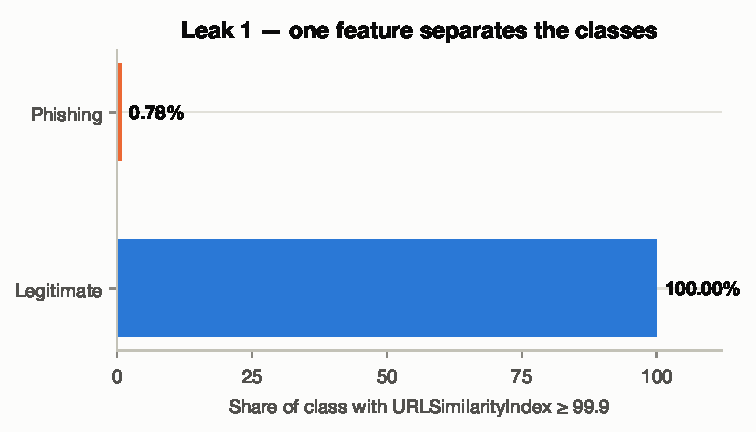
\includegraphics[width=0.72\textwidth]{figures/leak1_similarity_index.pdf}
\caption{One feature separates the classes almost perfectly. Any model given this column is
reporting the column's behaviour, not its own.}
\label{fig:leak1}
\end{figure}

\subsection{Leak 2: the classes were collected differently}

The second leak is structural and more damaging, because it is not confined to a column that can be
dropped. Table~\ref{tab:profile} profiles the two classes.

\begin{table}[h]
\centering
\begin{tabular}{lrr}
\toprule
Trait & Legitimate & Phishing \\
\midrule
Scheme is HTTPS & 100.00\,\% & 48.74\,\% \\
Host starts with \texttt{www.} & 100.00\,\% & 41.36\,\% \\
Has a path & 0.00\,\% & 28.42\,\% \\
Has a query string & 0.00\,\% & 6.08\,\% \\
Contains \texttt{@} & 0.00\,\% & 0.01\,\% \\
Mean URL length & 27.2 & 46.2 \\
\midrule
Rows & 134{,}850 & 100{,}945 \\
\bottomrule
\end{tabular}

\caption{Structural profile by class. Not one of the 134\,850 legitimate URLs has a path, a query
string or an \texttt{@}; every one uses HTTPS and a \texttt{www.} host.}
\label{tab:profile}
\end{table}

The legitimate set was normalised to \texttt{https://www.<domain>} when it was assembled; the
phishing set was written out verbatim from feeds. Consequently \emph{has a path} $\Rightarrow$
\emph{phishing} is \LeakTwoAcc{} accurate and, critically, has a false-positive rate of exactly zero
(Figure~\ref{fig:leak2}). A model with access to the raw URL string can reach very high accuracy by
learning which of two collection pipelines produced a row.

\begin{figure}[h]
\centering
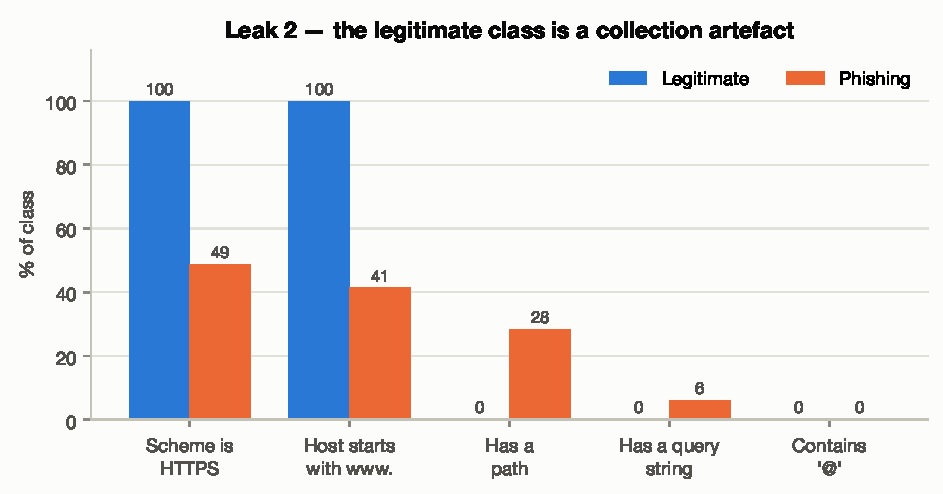
\includegraphics[width=0.86\textwidth]{figures/leak2_structural_profile.pdf}
\caption{Leak 2. The legitimate class is uniform on four independent traits, which is a property of
how it was gathered rather than of legitimate websites.}
\label{fig:leak2}
\end{figure}

\subsection{What the leaks are worth}

Table~\ref{tab:leakmodels} trains LightGBM on progressively cleaner feature sets, using the random
80/20 split that the literature uses.

\begin{table}[h]
\centering
\begin{tabular}{lr}
\toprule
Feature set & Accuracy \\
\midrule
All 50 precomputed features & 1.0000 \\
Minus \texttt{URLSimilarityIndex} & 1.0000 \\
Minus page-content columns (21 features) & 0.9973 \\
Hand-rolled lexical features on the raw URL & 0.9951 \\
\bottomrule
\end{tabular}

\caption{Accuracy under a random split. The last row is the important one: discarding every
precomputed column and engineering lexical features from the raw URL --- the correct instinct on
discovering leak 1 --- still yields \NaiveAcc{}, and still measures the collection artifact.}
\label{tab:leakmodels}
\end{table}

\section{Method}

\subsection{Canonicalisation}

Every URL is reduced to a canonical host name before anything else happens: lowercased, with the
scheme, userinfo, port, path, query, fragment, trailing dot and leading \texttt{www.} removed. This
is what neutralises leak 2, and it simultaneously removes a trap in the out-of-distribution
evaluation, where Tranco supplies bare domains and the phishing feeds supply deep URLs --- a
full-URL comparison there would reproduce the same ``has a path'' shortcut in a new setting.

The constraint is enforced mechanically rather than by discipline. A guard test mutates the scheme,
path, query, port and \texttt{www.} prefix of each URL in a corpus and asserts the feature vector is
bit-identical; a negative control plants such a leak and confirms the guard detects it.

\subsection{Features}

\NumFeatures{} features are computed from the host name alone, in four groups: \emph{shape} (host
and label lengths, subdomain depth), \emph{composition} (Shannon entropy, digit and hyphen ratios,
longest digit and consonant runs), \emph{structure} (IP literal, punycode, multi-level suffix,
provider-hosted), and \emph{lexical} (login-related keywords, brand tokens, and
\texttt{brand\_in\_subdomain\_only}, which fires on the \texttt{paypal.com.evil.tk} shape).

The top-level domain is one-hot encoded over the 25 most frequent suffixes rather than
target-encoded: a TLD phishing prior fitted on the data would reintroduce the label through the back
door. The brand vocabulary is frozen from the Tranco top 1000, which ranks by popularity and is
therefore label-independent by construction.

\subsection{Splitting}

Registrable domains are resolved against a frozen Public Suffix List snapshot and used as groups in
a \texttt{GroupShuffleSplit}, so no eTLD+1 appears on both sides of the split. \TrainHosts{} unique
hosts across \TrainGroups{} registrable domains remain after deduplication.

Only the ICANN section of the list is used for grouping. Under the private section
\texttt{evil.vercel.app} and \texttt{nice.vercel.app} would be distinct groups, letting the model be
rewarded at test time for memorising a hosting provider seen in training; grouping under ICANN
forces all of \texttt{vercel.app} to one side. Provider hosting is exposed as a feature instead,
which is where that signal can inform without inflating.

\subsection{Evaluation protocol}

Two regimes are reported. The \emph{internal hold-out} is the grouped split above. The
\emph{out-of-distribution and temporal} set pairs Tranco hosts with PhishTank hosts submitted after
2024-03-04, the date of the PhiUSIIL archive. Three contaminations are removed and counted
(Table~\ref{tab:oodcomp}), each of which would otherwise flatter the result --- most importantly the
42\,005 Tranco hosts that already appear in training, which would make 42\,\% of a naive benign
sample a memory test.

Hosts appearing on both a benign and a phishing list are excluded rather than arbitrated. They are
compromised legitimate sites hosting phishing content, a real phenomenon whose label is genuinely
ambiguous at the host level.

\begin{table}[h]
\centering
\begin{tabular}{lr}
\toprule
& Hosts \\
\midrule
Tranco hosts considered & 1{,}000{,}000 \\
PhishTank hosts (all) & 37{,}244 \\
PhishTank hosts after the cutoff & 31{,}726 \\
Removed: benign already seen in training & 42{,}005 \\
Removed: phishing already seen in training & 121 \\
Removed: host on both a benign and a phishing list & 267 \\
Final benign & 100{,}000 \\
Final phishing & 31{,}396 \\
OpenPhish probe hosts & 260 \\
\bottomrule
\end{tabular}

\caption{Composition of the out-of-distribution set, including every exclusion.}
\label{tab:oodcomp}
\end{table}

The primary metric is \textbf{recall at a fixed false-positive rate}. A false positive blocks a
legitimate site, which is the operationally expensive error, and accuracy on a near-balanced set
says nothing about behaviour at a usable operating point.

\section{Results}

\begin{table}[h]
\centering
\begin{tabular}{lrr}
\toprule
& Internal hold-out & OOD + temporal \\
\midrule
Hosts evaluated & 50{,}332 & 131{,}396 \\
Of which phishing & 23{,}424 & 31{,}396 \\
ROC-AUC & 0.9187 & 0.9372 \\
PR-AUC & 0.9345 & 0.9078 \\
Recall @ FPR 1\,\% & 72.59\,\% & 70.55\,\% \\
Recall @ FPR 0.1\,\% & 63.46\,\% & 50.78\,\% \\
Precision at operating point & 98.44\,\% & 95.68\,\% \\
$F_1$ at operating point & 0.8356 & 0.8122 \\
False positives & 269 / 26{,}908 & 999 / 100{,}000 \\
\bottomrule
\end{tabular}

\caption{Performance in both regimes. The operating point is the threshold achieving a 1\,\%
false-positive rate.}
\label{tab:results}
\end{table}

Table~\ref{tab:results} reports ROC-AUC \OodAuc{} and \OodRecall\,\% recall at 1\,\% false positives
out of distribution, against \InternalRecall\,\% internally. On the OpenPhish feed --- phishing URLs
that were live on the capture date and appear in no training data --- \OpenphishRate\,\% of hosts
are detected at the same threshold.

\begin{figure}[h]
\centering
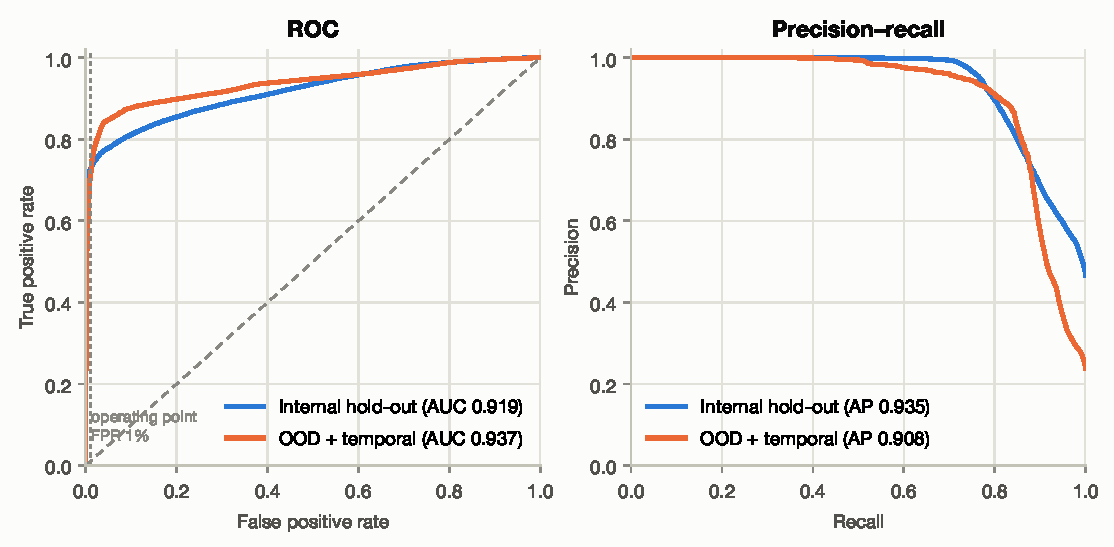
\includegraphics[width=\textwidth]{figures/roc_pr_curves.pdf}
\caption{ROC and precision--recall in both regimes. The dashed vertical line marks the 1\,\%
false-positive operating point.}
\label{fig:curves}
\end{figure}

That out-of-distribution ROC-AUC slightly exceeds the internal figure is worth stating plainly
rather than presenting as a success: the grouped internal split is the harder discrimination,
because PhiUSIIL's legitimate hosts are long-tail domains, whereas Tranco's benign set is dominated
by popular sites whose host names are short, dictionary-like and easy to separate. The two numbers
are not directly comparable, and neither is evidence that the model transfers well.

\subsection{Choosing the threshold}

At the default 0.5 threshold the model produces 13\,453 false positives on 100\,000 benign hosts.
At \OodThreshold{}, chosen from the ROC at a 1\,\% false-positive rate, it produces 999 --- a
92.6\,\% reduction --- at a cost of 18 points of recall. For a detector fronting real traffic this
is the correct side of the trade, and the service exposes both the threshold and its rationale.

\begin{figure}[h]
\centering
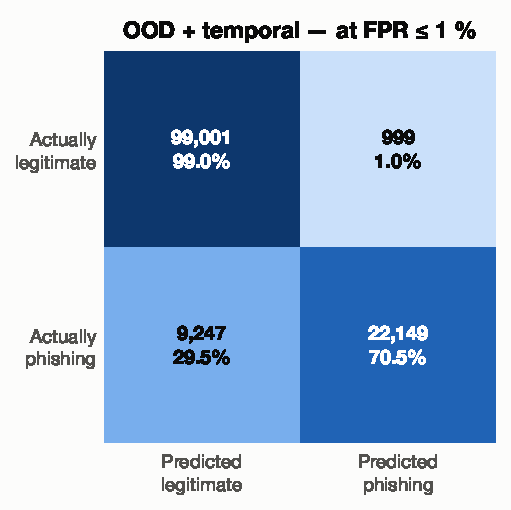
\includegraphics[width=0.55\textwidth]{figures/confusion_ood.pdf}
\caption{Confusion matrix out of distribution at the 1\,\% false-positive operating point.}
\label{fig:confusion}
\end{figure}

\subsection{What the model learned}

Figure~\ref{fig:shap} ranks features by mean absolute SHAP value over 4\,000
out-of-distribution hosts. Subdomain depth dominates, followed by digit count, the top-level domain
and subdomain length --- which is a coherent description of how phishing host names are actually
constructed: a recognisable-looking prefix stacked in front of a cheap registrable domain. The
twenty-six suffix indicators are summed into a single entry, which is exact because SHAP values are
additive.

Notably, the model is \emph{not} leaning on the hand-supplied lexical priors. The keyword list and
the brand features rank below the purely structural measurements, which suggests the structural
shape of a host name carries more signal than the presence of words a defender thought to enumerate.

\begin{figure}[h]
\centering
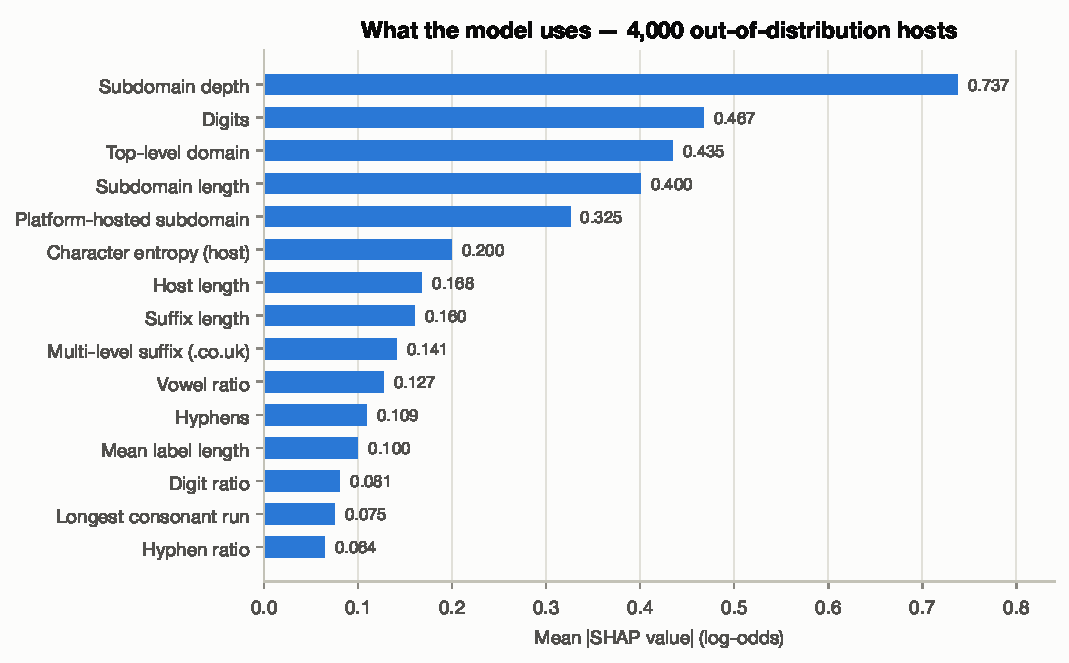
\includegraphics[width=0.82\textwidth]{figures/shap_global_importance.pdf}
\caption{Global feature importance on data the model never saw.}
\label{fig:shap}
\end{figure}

\section{Client-side scoring and explanation}

The public demonstration is a static page with no backend: it loads a 0.86\,MB pruned tree ensemble
and computes the prediction and its explanation locally. Explanations use path-dependent TreeSHAP
\cite{treeshap}, reimplemented in JavaScript.

An explanation computed by a reimplementation is only worth showing if it is the same computation.
Table~\ref{tab:parity} reports agreement between the JavaScript engine and the Python reference over
a corpus of \ParityUrls{} URLs spanning edge cases and samples from all four data sources.

\begin{table}[h]
\centering
\begin{tabular}{lrr}
\toprule
Compared & Count & Max.\ abs.\ difference \\
\midrule
Canonical hosts & 567 & exact \\
Feature values & 28{,}917 & $0$ \\
Raw scores & 567 & $0$ \\
SHAP attributions & 28{,}917 & $8.9\times 10^{-16}$ \\
SHAP additivity in JS & 567 & $1.9\times 10^{-13}$ \\
\bottomrule
\end{tabular}

\caption{Python versus JavaScript. Feature values and raw scores agree exactly; SHAP attributions
agree to machine precision. For reference, \texttt{shap}'s own additivity residual on this stack
measures $5\times10^{-16}$.}
\label{tab:parity}
\end{table}

A hash of the feature specification travels inside the model artifact, and the page refuses to score
if its own extractor disagrees --- making train/serve skew a visible failure rather than a quietly
wrong probability.

\begin{figure}[h]
\centering
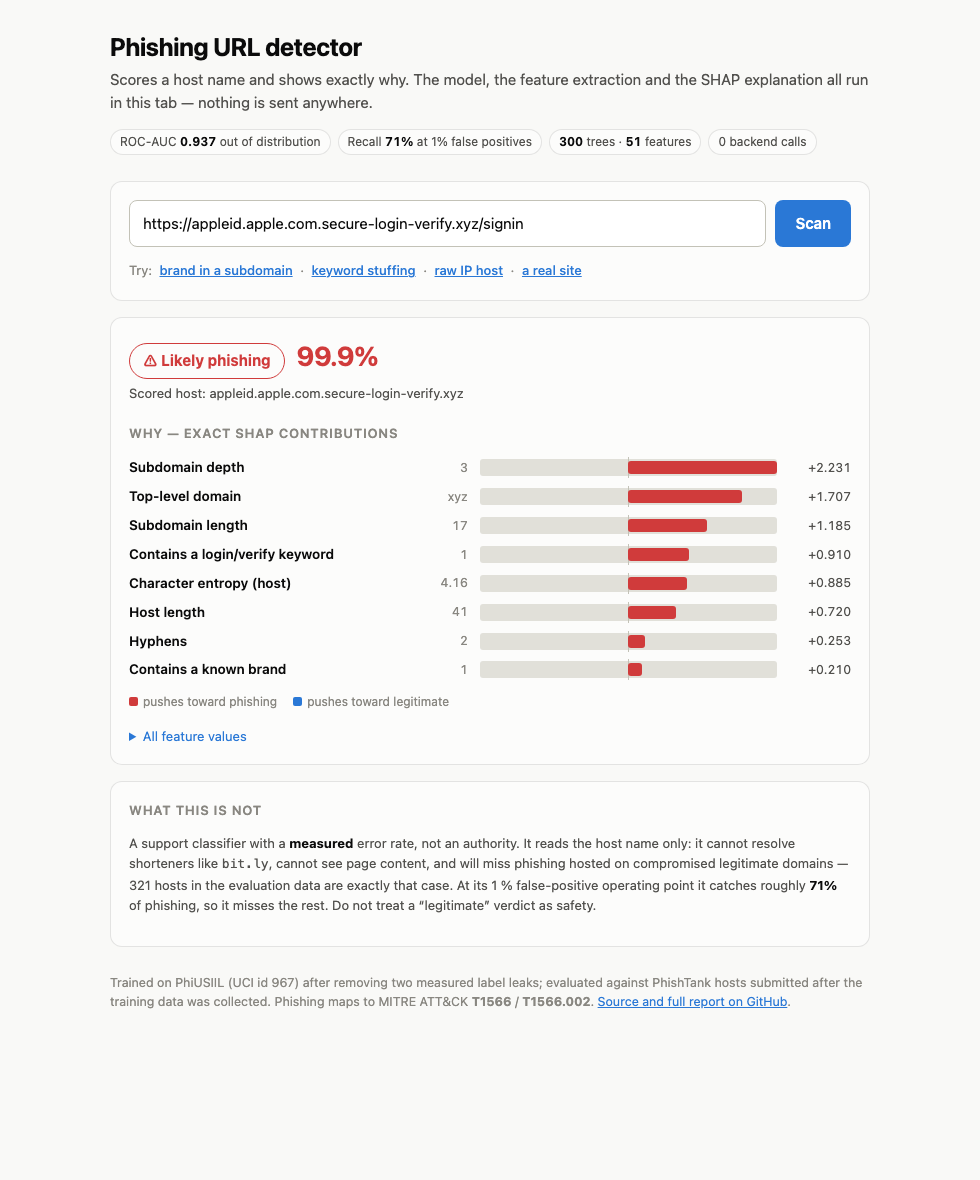
\includegraphics[width=0.86\textwidth]{figures/demo_phishing_light.png}
\caption{The deployed demonstration explaining a brand-impersonation host. The contributions shown
are exact: they sum, with the base value, to the model's log-odds output.}
\label{fig:demo}
\end{figure}

\section{Threat-model context}

Phishing links correspond to MITRE ATT\&CK technique \textbf{T1566} and sub-technique
\textbf{T1566.002} (Spearphishing Link) \cite{mitre}. The feature
\texttt{brand\_in\_subdomain\_only} directly targets the impersonation pattern in which a brand name
appears in the subdomain but not in the registrable domain, as in
\texttt{appleid.apple.com.secure-login-verify.xyz}, whose registrable domain is
\texttt{secure-login-verify.xyz}.

Detection logic lives in version control as tested feature definitions rather than as console
configuration, which makes it reviewable and diffable in the same way a Sigma rule or a query-based
detection would be.

\section{Limitations}

This is a support classifier with a measured error rate, not an authority.

It reads host names only. It cannot resolve URL shorteners, whose host is uninformative by design;
it cannot inspect page content; and it cannot detect phishing hosted on compromised legitimate
domains --- 267 hosts in the evaluation data are exactly that case, and were excluded from scoring
precisely because a host-level label cannot describe them. At the reported operating point it misses
roughly 30\,\% of phishing.

The benign proxy is a popularity ranking, which under-represents the long tail of small legitimate
sites; the false-positive rate on such sites is likely higher than the reported 1\,\%. The phishing
feeds are live and rotate, so the numbers here correspond to the 14 August 2026 capture.

\section{Conclusion}

A reported accuracy of \FullAcc{} on PhiUSIIL becomes \OodRecall\,\% recall at a 1\,\%
false-positive rate once two label leaks are removed and the model is confronted with phishing that
post-dates its training data by two years. The distance between those numbers is the contribution of
this report. The resulting model is smaller, weaker, and considerably more informative about what
lexical phishing detection can actually do.

\begin{thebibliography}{9}
\bibitem{phiusiil} A.~Prasad and S.~Chandra. \emph{PhiUSIIL: A Diverse Security Profile Empowered
Phishing URL Detection Framework}. Computers \& Security, 2024. UCI Machine Learning Repository,
dataset 967. \url{https://archive.ics.uci.edu/dataset/967}
\bibitem{tranco} V.~Le~Pochat et al. \emph{Tranco: A Research-Oriented Top Sites Ranking Hardened
Against Manipulation}. NDSS, 2019. \url{https://tranco-list.eu}
\bibitem{treeshap} S.~M.~Lundberg, G.~G.~Erion and S.-I.~Lee. \emph{Consistent Individualized
Feature Attribution for Tree Ensembles}. arXiv:1802.03888, 2018.
\bibitem{mitre} MITRE ATT\&CK. \emph{T1566: Phishing}; \emph{T1566.002: Spearphishing Link}.
\url{https://attack.mitre.org/techniques/T1566/}
\end{thebibliography}

\end{document}
